\documentclass[1p]{elsarticle_modified}
%\bibliographystyle{elsarticle-num}

%\usepackage[colorlinks]{hyperref}
%\usepackage{abbrmath_seonhwa} %\Abb, \Ascr, \Acal ,\Abf, \Afrak
\usepackage{amsfonts}
\usepackage{amssymb}
\usepackage{amsmath}
\usepackage{amsthm}
\usepackage{scalefnt}
\usepackage{amsbsy}
\usepackage{kotex}
\usepackage{caption}
\usepackage{subfig}
\usepackage{color}
\usepackage{graphicx}
\usepackage{xcolor} %% white, black, red, green, blue, cyan, magenta, yellow
\usepackage{float}
\usepackage{setspace}
\usepackage{hyperref}

\usepackage{tikz}
\usetikzlibrary{arrows}

\usepackage{multirow}
\usepackage{array} % fixed length table
\usepackage{hhline}

%%%%%%%%%%%%%%%%%%%%%
\makeatletter
\renewcommand*\env@matrix[1][\arraystretch]{%
	\edef\arraystretch{#1}%
	\hskip -\arraycolsep
	\let\@ifnextchar\new@ifnextchar
	\array{*\c@MaxMatrixCols c}}
\makeatother %https://tex.stackexchange.com/questions/14071/how-can-i-increase-the-line-spacing-in-a-matrix
%%%%%%%%%%%%%%%

\usepackage[normalem]{ulem}

\newcommand{\msout}[1]{\ifmmode\text{\sout{\ensuremath{#1}}}\else\sout{#1}\fi}
%SOURCE: \msout is \stkout macro in https://tex.stackexchange.com/questions/20609/strikeout-in-math-mode

\newcommand{\cancel}[1]{
	\ifmmode
	{\color{red}\msout{#1}}
	\else
	{\color{red}\sout{#1}}
	\fi
}

\newcommand{\add}[1]{
	{\color{blue}\uwave{#1}}
}

\newcommand{\replace}[2]{
	\ifmmode
	{\color{red}\msout{#1}}{\color{blue}\uwave{#2}}
	\else
	{\color{red}\sout{#1}}{\color{blue}\uwave{#2}}
	\fi
}

\newcommand{\Sol}{\mathcal{S}} %segment
\newcommand{\D}{D} %diagram
\newcommand{\A}{\mathcal{A}} %arc


%%%%%%%%%%%%%%%%%%%%%%%%%%%%%5 test

\def\sl{\operatorname{\textup{SL}}(2,\Cbb)}
\def\psl{\operatorname{\textup{PSL}}(2,\Cbb)}
\def\quan{\mkern 1mu \triangleright \mkern 1mu}

\theoremstyle{definition}
\newtheorem{thm}{Theorem}[section]
\newtheorem{prop}[thm]{Proposition}
\newtheorem{lem}[thm]{Lemma}
\newtheorem{ques}[thm]{Question}
\newtheorem{cor}[thm]{Corollary}
\newtheorem{defn}[thm]{Definition}
\newtheorem{exam}[thm]{Example}
\newtheorem{rmk}[thm]{Remark}
\newtheorem{alg}[thm]{Algorithm}

\newcommand{\I}{\sqrt{-1}}
\begin{document}

%\begin{frontmatter}
%
%\title{Boundary parabolic representations of knots up to 8 crossings}
%
%%% Group authors per affiliation:
%\author{Yunhi Cho} 
%\address{Department of Mathematics, University of Seoul, Seoul, Korea}
%\ead{yhcho@uos.ac.kr}
%
%
%\author{Seonhwa Kim} %\fnref{s_kim}}
%\address{Center for Geometry and Physics, Institute for Basic Science, Pohang, 37673, Korea}
%\ead{ryeona17@ibs.re.kr}
%
%\author{Hyuk Kim}
%\address{Department of Mathematical Sciences, Seoul National University, Seoul 08826, Korea}
%\ead{hyukkim@snu.ac.kr}
%
%\author{Seokbeom Yoon}
%\address{Department of Mathematical Sciences, Seoul National University, Seoul, 08826,  Korea}
%\ead{sbyoon15@snu.ac.kr}
%
%\begin{abstract}
%We find all boundary parabolic representation of knots up to 8 crossings.
%
%\end{abstract}
%\begin{keyword}
%    \MSC[2010] 57M25 
%\end{keyword}
%
%\end{frontmatter}

%\linenumbers
%\tableofcontents
%
\newcommand\colored[1]{\textcolor{white}{\rule[-0.35ex]{0.8em}{1.4ex}}\kern-0.8em\color{red} #1}%
%\newcommand\colored[1]{\textcolor{white}{ #1}\kern-2.17ex	\textcolor{white}{ #1}\kern-1.81ex	\textcolor{white}{ #1}\kern-2.15ex\color{red}#1	}

{\Large $\underline{12a_{0664}~(K12a_{0664})}$}

\setlength{\tabcolsep}{10pt}
\renewcommand{\arraystretch}{1.6}
\vspace{1cm}\begin{tabular}{m{100pt}>{\centering\arraybackslash}m{274pt}}
\multirow{5}{120pt}{
	\centering
	\includegraphics[width=112pt]{../../../GIT/diagram.site/Diagrams/png/1465_12a_0664.png}\\
\ \ \ A knot diagram\footnotemark}&
\allowdisplaybreaks
\textbf{Linearized knot diagam} \\
\cline{2-2}
 &
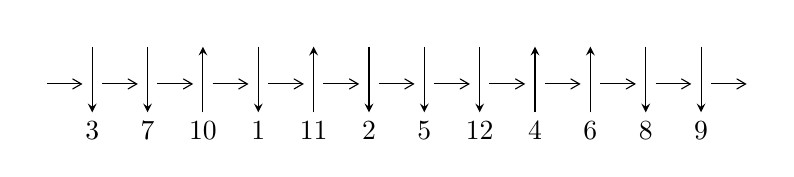
\begin{tikzpicture}[x=20pt, y=17pt]
	% nodes
	\node (C0) at (0, 0) {};
	\node (C1) at (1, 0) {};
	\node (C1U) at (1, +1) {};
	\node (C1D) at (1, -1) {3};

	\node (C2) at (2, 0) {};
	\node (C2U) at (2, +1) {};
	\node (C2D) at (2, -1) {7};

	\node (C3) at (3, 0) {};
	\node (C3U) at (3, +1) {};
	\node (C3D) at (3, -1) {10};

	\node (C4) at (4, 0) {};
	\node (C4U) at (4, +1) {};
	\node (C4D) at (4, -1) {1};

	\node (C5) at (5, 0) {};
	\node (C5U) at (5, +1) {};
	\node (C5D) at (5, -1) {11};

	\node (C6) at (6, 0) {};
	\node (C6U) at (6, +1) {};
	\node (C6D) at (6, -1) {2};

	\node (C7) at (7, 0) {};
	\node (C7U) at (7, +1) {};
	\node (C7D) at (7, -1) {5};

	\node (C8) at (8, 0) {};
	\node (C8U) at (8, +1) {};
	\node (C8D) at (8, -1) {12};

	\node (C9) at (9, 0) {};
	\node (C9U) at (9, +1) {};
	\node (C9D) at (9, -1) {4};

	\node (C10) at (10, 0) {};
	\node (C10U) at (10, +1) {};
	\node (C10D) at (10, -1) {6};

	\node (C11) at (11, 0) {};
	\node (C11U) at (11, +1) {};
	\node (C11D) at (11, -1) {8};

	\node (C12) at (12, 0) {};
	\node (C12U) at (12, +1) {};
	\node (C12D) at (12, -1) {9};
	\node (C13) at (13, 0) {};

	% arrows
	\draw[->,>={angle 60}]
	(C0) edge (C1) (C1) edge (C2) (C2) edge (C3) (C3) edge (C4) (C4) edge (C5) (C5) edge (C6) (C6) edge (C7) (C7) edge (C8) (C8) edge (C9) (C9) edge (C10) (C10) edge (C11) (C11) edge (C12) (C12) edge (C13) ;	\draw[->,>=stealth]
	(C1U) edge (C1D) (C2U) edge (C2D) (C3D) edge (C3U) (C4U) edge (C4D) (C5D) edge (C5U) (C6U) edge (C6D) (C7U) edge (C7D) (C8U) edge (C8D) (C9D) edge (C9U) (C10D) edge (C10U) (C11U) edge (C11D) (C12U) edge (C12D) ;
	\end{tikzpicture} \\
\hhline{~~} \\& 
\textbf{Solving Sequence} \\ \cline{2-2} 
 &
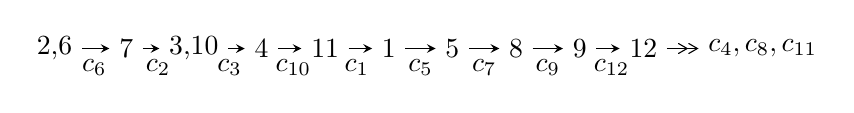
\begin{tikzpicture}[x=23pt, y=7pt]
	% node
	\node (A0) at (-1/8, 0) {2,6};
	\node (A1) at (1, 0) {7};
	\node (A2) at (33/16, 0) {3,10};
	\node (A3) at (25/8, 0) {4};
	\node (A4) at (33/8, 0) {11};
	\node (A5) at (41/8, 0) {1};
	\node (A6) at (49/8, 0) {5};
	\node (A7) at (57/8, 0) {8};
	\node (A8) at (65/8, 0) {9};
	\node (A9) at (73/8, 0) {12};
	\node (C1) at (1/2, -1) {$c_{6}$};
	\node (C2) at (3/2, -1) {$c_{2}$};
	\node (C3) at (21/8, -1) {$c_{3}$};
	\node (C4) at (29/8, -1) {$c_{10}$};
	\node (C5) at (37/8, -1) {$c_{1}$};
	\node (C6) at (45/8, -1) {$c_{5}$};
	\node (C7) at (53/8, -1) {$c_{7}$};
	\node (C8) at (61/8, -1) {$c_{9}$};
	\node (C9) at (69/8, -1) {$c_{12}$};
	\node (A10) at (11, 0) {$c_{4},c_{8},c_{11}$};

	% edge
	\draw[->,>=stealth]	
	(A0) edge (A1) (A1) edge (A2) (A2) edge (A3) (A3) edge (A4) (A4) edge (A5) (A5) edge (A6) (A6) edge (A7) (A7) edge (A8) (A8) edge (A9) ;
	\draw[->>,>={angle 60}]	
	(A9) edge (A10);
\end{tikzpicture} \\ 

\end{tabular} \\

\footnotetext{
The image of knot diagram is generated by the software ``\textbf{Draw programme}" developed by Andrew Bartholomew(\url{http://www.layer8.co.uk/maths/draw/index.htm\#Running-draw}), where we modified some parts for our purpose(\url{https://github.com/CATsTAILs/LinksPainter}).
}\phantom \\ \newline 
\centering \textbf{Ideals for irreducible components\footnotemark of $X_{\text{par}}$} 
 
\begin{align*}
I^u_{1}&=\langle 
-1185 u^{34}+14000 u^{33}+\cdots+32 b+15808,\;3556 u^{34}-45981 u^{33}+\cdots+32 a+144096,\\
\phantom{I^u_{1}}&\phantom{= \langle  }u^{35}-14 u^{34}+\cdots+608 u-64\rangle \\
I^u_{2}&=\langle 
1.49681\times10^{45} a^{11} u^{5}-5.70342\times10^{45} a^{10} u^{5}+\cdots-1.15780\times10^{47} a+2.97901\times10^{46},\\
\phantom{I^u_{2}}&\phantom{= \langle  }- a^{11} u^5-4 a^{10} u^5+\cdots-55 a-18,\;u^6+u^5- u^4-2 u^3+u+1\rangle \\
I^u_{3}&=\langle 
-2 u^{22}+11 u^{20}+\cdots+b-8,\;9 u^{22}+8 u^{21}+\cdots+a+17,\;u^{23}+u^{22}+\cdots+3 u+1\rangle \\
\\
\end{align*}
\raggedright * 3 irreducible components of $\dim_{\mathbb{C}}=0$, with total 130 representations.\\
\footnotetext{All coefficients of polynomials are rational numbers. But the coefficients are sometimes approximated in decimal forms when there is not enough margin.}
\newpage
\renewcommand{\arraystretch}{1}
\centering \section*{I. $I^u_{1}= \langle -1185 u^{34}+14000 u^{33}+\cdots+32 b+15808,\;3556 u^{34}-45981 u^{33}+\cdots+32 a+144096,\;u^{35}-14 u^{34}+\cdots+608 u-64 \rangle$}
\flushleft \textbf{(i) Arc colorings}\\
\begin{tabular}{m{7pt} m{180pt} m{7pt} m{180pt} }
\flushright $a_{2}=$&$\begin{pmatrix}0\\u\end{pmatrix}$ \\
\flushright $a_{6}=$&$\begin{pmatrix}1\\0\end{pmatrix}$ \\
\flushright $a_{7}=$&$\begin{pmatrix}1\\u^2\end{pmatrix}$ \\
\flushright $a_{3}=$&$\begin{pmatrix}- u\\- u^3+u\end{pmatrix}$ \\
\flushright $a_{10}=$&$\begin{pmatrix}-111.125 u^{34}+1436.91 u^{33}+\cdots+41697.5 u-4503\\\frac{1185}{32} u^{34}-\frac{875}{2} u^{33}+\cdots+2084 u-494\end{pmatrix}$ \\
\flushright $a_{4}=$&$\begin{pmatrix}\frac{1045}{64} u^{34}-\frac{1759}{8} u^{33}+\cdots-\frac{37185}{4} u+1064\\-\frac{541}{32} u^{34}+\frac{847}{4} u^{33}+\cdots+\frac{9217}{2} u-487\end{pmatrix}$ \\
\flushright $a_{11}=$&$\begin{pmatrix}-74.0938 u^{34}+999.406 u^{33}+\cdots+43781.5 u-4997\\\frac{1185}{32} u^{34}-\frac{875}{2} u^{33}+\cdots+2084 u-494\end{pmatrix}$ \\
\flushright $a_{1}=$&$\begin{pmatrix}u^3\\u^5- u^3+u\end{pmatrix}$ \\
\flushright $a_{5}=$&$\begin{pmatrix}\frac{37}{64} u^{34}+\frac{65}{8} u^{33}+\cdots+\frac{18751}{4} u-576\\\frac{541}{32} u^{34}-\frac{847}{4} u^{33}+\cdots-\frac{9215}{2} u+487\end{pmatrix}$ \\
\flushright $a_{8}=$&$\begin{pmatrix}\frac{211}{8} u^{34}-\frac{11137}{32} u^{33}+\cdots-13901 u+\frac{3187}{2}\\\frac{279}{32} u^{34}-\frac{2045}{16} u^{33}+\cdots-\frac{17517}{2} u+1046\end{pmatrix}$ \\
\flushright $a_{9}=$&$\begin{pmatrix}\frac{865}{64} u^{34}-\frac{1229}{8} u^{33}+\cdots-2691 u+\frac{667}{2}\\56.2188 u^{34}-774.938 u^{33}+\cdots-36723 u+4223\end{pmatrix}$ \\
\flushright $a_{12}=$&$\begin{pmatrix}12.7813 u^{34}-135.594 u^{33}+\cdots+2973.50 u-394.500\\\frac{1685}{32} u^{34}-\frac{5693}{8} u^{33}+\cdots-\frac{58715}{2} u+3332\end{pmatrix}$\\&\end{tabular}
\flushleft \textbf{(ii) Obstruction class $= -1$}\\~\\
\flushleft \textbf{(iii) Cusp Shapes $= -\frac{459}{2} u^{34}+3017 u^{33}+\cdots+110596 u-12350$}\\~\\
\newpage\renewcommand{\arraystretch}{1}
\flushleft \textbf{(iv) u-Polynomials at the component}\newline \\
\begin{tabular}{m{50pt}|m{274pt}}
Crossings & \hspace{64pt}u-Polynomials at each crossing \\
\hline $$\begin{aligned}c_{1}\end{aligned}$$&$\begin{aligned}
&u^{35}+12 u^{34}+\cdots+13312 u+4096
\end{aligned}$\\
\hline $$\begin{aligned}c_{2},c_{6}\end{aligned}$$&$\begin{aligned}
&u^{35}-14 u^{34}+\cdots+608 u-64
\end{aligned}$\\
\hline $$\begin{aligned}c_{3},c_{5},c_{9}\\c_{10}\end{aligned}$$&$\begin{aligned}
&u^{35}+14 u^{33}+\cdots-4 u-1
\end{aligned}$\\
\hline $$\begin{aligned}c_{4},c_{7}\end{aligned}$$&$\begin{aligned}
&u^{35}-2 u^{34}+\cdots+9 u-1
\end{aligned}$\\
\hline $$\begin{aligned}c_{8},c_{11},c_{12}\end{aligned}$$&$\begin{aligned}
&u^{35}+16 u^{34}+\cdots+160 u-64
\end{aligned}$\\
\hline
\end{tabular}\\~\\
\newpage\renewcommand{\arraystretch}{1}
\flushleft \textbf{(v) Riley Polynomials at the component}\newline \\
\begin{tabular}{m{50pt}|m{274pt}}
Crossings & \hspace{64pt}Riley Polynomials at each crossing \\
\hline $$\begin{aligned}c_{1}\end{aligned}$$&$\begin{aligned}
&y^{35}+8 y^{34}+\cdots-158334976 y-16777216
\end{aligned}$\\
\hline $$\begin{aligned}c_{2},c_{6}\end{aligned}$$&$\begin{aligned}
&y^{35}-12 y^{34}+\cdots+13312 y-4096
\end{aligned}$\\
\hline $$\begin{aligned}c_{3},c_{5},c_{9}\\c_{10}\end{aligned}$$&$\begin{aligned}
&y^{35}+28 y^{34}+\cdots+6 y-1
\end{aligned}$\\
\hline $$\begin{aligned}c_{4},c_{7}\end{aligned}$$&$\begin{aligned}
&y^{35}-12 y^{34}+\cdots+135 y-1
\end{aligned}$\\
\hline $$\begin{aligned}c_{8},c_{11},c_{12}\end{aligned}$$&$\begin{aligned}
&y^{35}-34 y^{34}+\cdots+54272 y-4096
\end{aligned}$\\
\hline
\end{tabular}\\~\\
\newpage\flushleft \textbf{(vi) Complex Volumes and Cusp Shapes}
$$\begin{array}{c|c|c}  
\text{Solutions to }I^u_{1}& \I (\text{vol} + \sqrt{-1}CS) & \text{Cusp shape}\\
 \hline 
\begin{aligned}
u &= -0.998696\phantom{ +0.000000I} \\
a &= \phantom{-}0.406523\phantom{ +0.000000I} \\
b &= \phantom{-}0.811456\phantom{ +0.000000I}\end{aligned}
 & -7.46368\phantom{ +0.000000I} & -11.8760\phantom{ +0.000000I} \\ \hline\begin{aligned}
u &= \phantom{-}0.735848 + 0.635706 I \\
a &= -1.072540 - 0.169141 I \\
b &= \phantom{-}0.692633 - 0.220382 I\end{aligned}
 & \phantom{-}2.59000 - 1.09744 I & \phantom{-0.000000 } 0 \\ \hline\begin{aligned}
u &= \phantom{-}0.735848 - 0.635706 I \\
a &= -1.072540 + 0.169141 I \\
b &= \phantom{-}0.692633 + 0.220382 I\end{aligned}
 & \phantom{-}2.59000 + 1.09744 I & \phantom{-0.000000 } 0 \\ \hline\begin{aligned}
u &= \phantom{-}0.388780 + 0.979792 I \\
a &= -0.611938 - 1.089240 I \\
b &= \phantom{-}0.49548 + 1.43787 I\end{aligned}
 & -11.7814 + 11.4404 I & \phantom{-0.000000 } 0 \\ \hline\begin{aligned}
u &= \phantom{-}0.388780 - 0.979792 I \\
a &= -0.611938 + 1.089240 I \\
b &= \phantom{-}0.49548 - 1.43787 I\end{aligned}
 & -11.7814 - 11.4404 I & \phantom{-0.000000 } 0 \\ \hline\begin{aligned}
u &= \phantom{-}0.331775 + 1.023800 I \\
a &= \phantom{-}0.554343 + 0.837484 I \\
b &= -0.415463 - 1.254440 I\end{aligned}
 & -3.76301 + 7.52599 I & \phantom{-0.000000 } 0 \\ \hline\begin{aligned}
u &= \phantom{-}0.331775 - 1.023800 I \\
a &= \phantom{-}0.554343 - 0.837484 I \\
b &= -0.415463 + 1.254440 I\end{aligned}
 & -3.76301 - 7.52599 I & \phantom{-0.000000 } 0 \\ \hline\begin{aligned}
u &= \phantom{-}0.897454 + 0.638918 I \\
a &= \phantom{-}0.670730 + 0.645138 I \\
b &= -0.663183 + 0.017922 I\end{aligned}
 & \phantom{-}2.11864 - 3.86118 I & \phantom{-0.000000 } 0 \\ \hline\begin{aligned}
u &= \phantom{-}0.897454 - 0.638918 I \\
a &= \phantom{-}0.670730 - 0.645138 I \\
b &= -0.663183 - 0.017922 I\end{aligned}
 & \phantom{-}2.11864 + 3.86118 I & \phantom{-0.000000 } 0 \\ \hline\begin{aligned}
u &= \phantom{-}0.978827 + 0.600935 I \\
a &= -0.829355 - 1.080510 I \\
b &= \phantom{-}0.938507 - 0.064693 I\end{aligned}
 & -3.98603 - 5.50029 I & \phantom{-0.000000 } 0\\
 \hline 
 \end{array}$$\newpage$$\begin{array}{c|c|c}  
\text{Solutions to }I^u_{1}& \I (\text{vol} + \sqrt{-1}CS) & \text{Cusp shape}\\
 \hline 
\begin{aligned}
u &= \phantom{-}0.978827 - 0.600935 I \\
a &= -0.829355 + 1.080510 I \\
b &= \phantom{-}0.938507 + 0.064693 I\end{aligned}
 & -3.98603 + 5.50029 I & \phantom{-0.000000 } 0 \\ \hline\begin{aligned}
u &= -0.838763\phantom{ +0.000000I} \\
a &= -0.220144\phantom{ +0.000000I} \\
b &= -0.339524\phantom{ +0.000000I}\end{aligned}
 & -1.49579\phantom{ +0.000000I} & -4.76650\phantom{ +0.000000I} \\ \hline\begin{aligned}
u &= \phantom{-}0.557853 + 0.610862 I \\
a &= \phantom{-}1.42477 + 0.11204 I \\
b &= -0.890998 + 0.031259 I\end{aligned}
 & -2.81360 + 0.71268 I & -3.56704 + 0.25723 I \\ \hline\begin{aligned}
u &= \phantom{-}0.557853 - 0.610862 I \\
a &= \phantom{-}1.42477 - 0.11204 I \\
b &= -0.890998 - 0.031259 I\end{aligned}
 & -2.81360 - 0.71268 I & -3.56704 - 0.25723 I \\ \hline\begin{aligned}
u &= \phantom{-}0.875442 + 0.817929 I \\
a &= \phantom{-}0.419001 - 0.418160 I \\
b &= -0.069182 + 0.582688 I\end{aligned}
 & \phantom{-}1.43497 - 3.03675 I & \phantom{-0.000000 } 0 \\ \hline\begin{aligned}
u &= \phantom{-}0.875442 - 0.817929 I \\
a &= \phantom{-}0.419001 + 0.418160 I \\
b &= -0.069182 - 0.582688 I\end{aligned}
 & \phantom{-}1.43497 + 3.03675 I & \phantom{-0.000000 } 0 \\ \hline\begin{aligned}
u &= \phantom{-}0.657165 + 1.106850 I \\
a &= -0.261979 + 0.777037 I \\
b &= \phantom{-}0.109636 - 1.218180 I\end{aligned}
 & -9.91255 - 5.35177 I & \phantom{-0.000000 } 0 \\ \hline\begin{aligned}
u &= \phantom{-}0.657165 - 1.106850 I \\
a &= -0.261979 - 0.777037 I \\
b &= \phantom{-}0.109636 + 1.218180 I\end{aligned}
 & -9.91255 + 5.35177 I & \phantom{-0.000000 } 0 \\ \hline\begin{aligned}
u &= \phantom{-}0.347142 + 1.298210 I \\
a &= -0.190435 - 0.549260 I \\
b &= \phantom{-}0.146118 + 1.125760 I\end{aligned}
 & -2.07712 + 1.05602 I & \phantom{-0.000000 } 0 \\ \hline\begin{aligned}
u &= \phantom{-}0.347142 - 1.298210 I \\
a &= -0.190435 + 0.549260 I \\
b &= \phantom{-}0.146118 - 1.125760 I\end{aligned}
 & -2.07712 - 1.05602 I & \phantom{-0.000000 } 0\\
 \hline 
 \end{array}$$\newpage$$\begin{array}{c|c|c}  
\text{Solutions to }I^u_{1}& \I (\text{vol} + \sqrt{-1}CS) & \text{Cusp shape}\\
 \hline 
\begin{aligned}
u &= \phantom{-}0.650933\phantom{ +0.000000I} \\
a &= \phantom{-}2.00998\phantom{ +0.000000I} \\
b &= -0.456707\phantom{ +0.000000I}\end{aligned}
 & -2.54150\phantom{ +0.000000I} & \phantom{-}4.22040\phantom{ +0.000000I} \\ \hline\begin{aligned}
u &= \phantom{-}1.184660 + 0.653764 I \\
a &= \phantom{-}1.76258 + 0.22362 I \\
b &= -0.56794 + 1.53123 I\end{aligned}
 & -14.2397 - 17.3604 I & \phantom{-0.000000 } 0 \\ \hline\begin{aligned}
u &= \phantom{-}1.184660 - 0.653764 I \\
a &= \phantom{-}1.76258 - 0.22362 I \\
b &= -0.56794 - 1.53123 I\end{aligned}
 & -14.2397 + 17.3604 I & \phantom{-0.000000 } 0 \\ \hline\begin{aligned}
u &= -1.351080 + 0.086351 I \\
a &= -0.133127 + 0.458938 I \\
b &= -0.27517 + 1.49696 I\end{aligned}
 & -18.1528 - 7.9861 I & \phantom{-0.000000 } 0 \\ \hline\begin{aligned}
u &= -1.351080 - 0.086351 I \\
a &= -0.133127 - 0.458938 I \\
b &= -0.27517 - 1.49696 I\end{aligned}
 & -18.1528 + 7.9861 I & \phantom{-0.000000 } 0 \\ \hline\begin{aligned}
u &= \phantom{-}1.209310 + 0.645834 I \\
a &= -1.55266 - 0.28086 I \\
b &= \phantom{-}0.51192 - 1.37648 I\end{aligned}
 & -6.4732 - 13.5026 I & \phantom{-0.000000 } 0 \\ \hline\begin{aligned}
u &= \phantom{-}1.209310 - 0.645834 I \\
a &= -1.55266 + 0.28086 I \\
b &= \phantom{-}0.51192 + 1.37648 I\end{aligned}
 & -6.4732 + 13.5026 I & \phantom{-0.000000 } 0 \\ \hline\begin{aligned}
u &= -0.298877 + 0.500011 I \\
a &= -0.622450 + 0.276097 I \\
b &= \phantom{-}0.134554 + 0.535427 I\end{aligned}
 & -0.168508 + 1.117130 I & -2.41743 - 5.24581 I \\ \hline\begin{aligned}
u &= -0.298877 - 0.500011 I \\
a &= -0.622450 - 0.276097 I \\
b &= \phantom{-}0.134554 - 0.535427 I\end{aligned}
 & -0.168508 - 1.117130 I & -2.41743 + 5.24581 I \\ \hline\begin{aligned}
u &= \phantom{-}1.27152 + 0.65655 I \\
a &= \phantom{-}1.227090 + 0.241685 I \\
b &= -0.350162 + 1.222410 I\end{aligned}
 & -5.27078 - 7.68372 I & \phantom{-0.000000 } 0\\
 \hline 
 \end{array}$$\newpage$$\begin{array}{c|c|c}  
\text{Solutions to }I^u_{1}& \I (\text{vol} + \sqrt{-1}CS) & \text{Cusp shape}\\
 \hline 
\begin{aligned}
u &= \phantom{-}1.27152 - 0.65655 I \\
a &= \phantom{-}1.227090 - 0.241685 I \\
b &= -0.350162 - 1.222410 I\end{aligned}
 & -5.27078 + 7.68372 I & \phantom{-0.000000 } 0 \\ \hline\begin{aligned}
u &= -1.44729 + 0.08376 I \\
a &= \phantom{-}0.070621 - 0.374099 I \\
b &= \phantom{-}0.127609 - 1.345440 I\end{aligned}
 & -10.28340 - 3.40903 I & \phantom{-0.000000 } 0 \\ \hline\begin{aligned}
u &= -1.44729 - 0.08376 I \\
a &= \phantom{-}0.070621 + 0.374099 I \\
b &= \phantom{-}0.127609 + 1.345440 I\end{aligned}
 & -10.28340 + 3.40903 I & \phantom{-0.000000 } 0 \\ \hline\begin{aligned}
u &= \phantom{-}1.25473 + 0.80657 I \\
a &= -0.952835 + 0.203116 I \\
b &= \phantom{-}0.068034 - 1.227290 I\end{aligned}
 & -11.81200 - 1.77127 I & \phantom{-0.000000 } 0 \\ \hline\begin{aligned}
u &= \phantom{-}1.25473 - 0.80657 I \\
a &= -0.952835 - 0.203116 I \\
b &= \phantom{-}0.068034 + 1.227290 I\end{aligned}
 & -11.81200 + 1.77127 I & \phantom{-0.000000 } 0\\
 \hline 
 \end{array}$$\newpage\newpage\renewcommand{\arraystretch}{1}
\centering \section*{II. $I^u_{2}= \langle 1.50\times10^{45} a^{11} u^{5}-5.70\times10^{45} a^{10} u^{5}+\cdots-1.16\times10^{47} a+2.98\times10^{46},\;- a^{11} u^5-4 a^{10} u^5+\cdots-55 a-18,\;u^6+u^5- u^4-2 u^3+u+1 \rangle$}
\flushleft \textbf{(i) Arc colorings}\\
\begin{tabular}{m{7pt} m{180pt} m{7pt} m{180pt} }
\flushright $a_{2}=$&$\begin{pmatrix}0\\u\end{pmatrix}$ \\
\flushright $a_{6}=$&$\begin{pmatrix}1\\0\end{pmatrix}$ \\
\flushright $a_{7}=$&$\begin{pmatrix}1\\u^2\end{pmatrix}$ \\
\flushright $a_{3}=$&$\begin{pmatrix}- u\\- u^3+u\end{pmatrix}$ \\
\flushright $a_{10}=$&$\begin{pmatrix}a\\-0.00794015 a^{11} u^{5}+0.0302550 a^{10} u^{5}+\cdots+0.614182 a-0.158028\end{pmatrix}$ \\
\flushright $a_{4}=$&$\begin{pmatrix}0.00490869 a^{11} u^{5}+0.0130821 a^{10} u^{5}+\cdots+0.785397 a+0.523477\\-0.00830184 a^{11} u^{5}+0.0195054 a^{10} u^{5}+\cdots-0.000748132 a-0.539669\end{pmatrix}$ \\
\flushright $a_{11}=$&$\begin{pmatrix}-0.00794015 a^{11} u^{5}+0.0302550 a^{10} u^{5}+\cdots+1.61418 a-0.158028\\-0.00794015 a^{11} u^{5}+0.0302550 a^{10} u^{5}+\cdots+0.614182 a-0.158028\end{pmatrix}$ \\
\flushright $a_{1}=$&$\begin{pmatrix}u^3\\u^5- u^3+u\end{pmatrix}$ \\
\flushright $a_{5}=$&$\begin{pmatrix}0.0247380 a^{11} u^{5}+0.0248517 a^{10} u^{5}+\cdots+0.0454023 a+0.368349\\0.00587845 a^{11} u^{5}+0.0341246 a^{10} u^{5}+\cdots+1.25016 a-1.03661\end{pmatrix}$ \\
\flushright $a_{8}=$&$\begin{pmatrix}0.00249911 a^{11} u^{5}-0.00445033 a^{10} u^{5}+\cdots+0.152457 a+0.669472\\0.0198608 a^{11} u^{5}-0.00986522 a^{10} u^{5}+\cdots-1.05246 a+0.630579\end{pmatrix}$ \\
\flushright $a_{9}=$&$\begin{pmatrix}-0.0209774 a^{11} u^{5}+0.0278972 a^{10} u^{5}+\cdots+0.449873 a-1.39397\\0.0146417 a^{11} u^{5}+0.0451106 a^{10} u^{5}+\cdots+0.588854 a-0.425328\end{pmatrix}$ \\
\flushright $a_{12}=$&$\begin{pmatrix}0.0432844 a^{11} u^{5}+0.0323424 a^{10} u^{5}+\cdots-1.19997 a+0.605993\\-0.0459402 a^{11} u^{5}+0.0636298 a^{10} u^{5}+\cdots+1.26067 a+0.107121\end{pmatrix}$\\&\end{tabular}
\flushleft \textbf{(ii) Obstruction class $= -1$}\\~\\
\flushleft \textbf{(iii) Cusp Shapes $= 0.0983999 a^{11} u^{5}-0.0411031 a^{10} u^{5}+\cdots-4.19581 a-8.39076$}\\~\\
\newpage\renewcommand{\arraystretch}{1}
\flushleft \textbf{(iv) u-Polynomials at the component}\newline \\
\begin{tabular}{m{50pt}|m{274pt}}
Crossings & \hspace{64pt}u-Polynomials at each crossing \\
\hline $$\begin{aligned}c_{1}\end{aligned}$$&$\begin{aligned}
&(u^6+3 u^5+5 u^4+4 u^3+2 u^2+u+1)^{12}
\end{aligned}$\\
\hline $$\begin{aligned}c_{2},c_{6}\end{aligned}$$&$\begin{aligned}
&(u^6+u^5- u^4-2 u^3+u+1)^{12}
\end{aligned}$\\
\hline $$\begin{aligned}c_{3},c_{5},c_{9}\\c_{10}\end{aligned}$$&$\begin{aligned}
&u^{72}+u^{71}+\cdots-23968 u+5312
\end{aligned}$\\
\hline $$\begin{aligned}c_{4},c_{7}\end{aligned}$$&$\begin{aligned}
&u^{72}-7 u^{71}+\cdots-872320 u+141376
\end{aligned}$\\
\hline $$\begin{aligned}c_{8},c_{11},c_{12}\end{aligned}$$&$\begin{aligned}
&(u^6- u^5-3 u^4+2 u^3+2 u^2+u-1)^{12}
\end{aligned}$\\
\hline
\end{tabular}\\~\\
\newpage\renewcommand{\arraystretch}{1}
\flushleft \textbf{(v) Riley Polynomials at the component}\newline \\
\begin{tabular}{m{50pt}|m{274pt}}
Crossings & \hspace{64pt}Riley Polynomials at each crossing \\
\hline $$\begin{aligned}c_{1}\end{aligned}$$&$\begin{aligned}
&(y^6+y^5+5 y^4+6 y^2+3 y+1)^{12}
\end{aligned}$\\
\hline $$\begin{aligned}c_{2},c_{6}\end{aligned}$$&$\begin{aligned}
&(y^6-3 y^5+5 y^4-4 y^3+2 y^2- y+1)^{12}
\end{aligned}$\\
\hline $$\begin{aligned}c_{3},c_{5},c_{9}\\c_{10}\end{aligned}$$&$\begin{aligned}
&y^{72}+63 y^{71}+\cdots+1187419136 y+28217344
\end{aligned}$\\
\hline $$\begin{aligned}c_{4},c_{7}\end{aligned}$$&$\begin{aligned}
&y^{72}-33 y^{71}+\cdots-667358056448 y+19987173376
\end{aligned}$\\
\hline $$\begin{aligned}c_{8},c_{11},c_{12}\end{aligned}$$&$\begin{aligned}
&(y^6-7 y^5+17 y^4-16 y^3+6 y^2-5 y+1)^{12}
\end{aligned}$\\
\hline
\end{tabular}\\~\\
\newpage\flushleft \textbf{(vi) Complex Volumes and Cusp Shapes}
$$\begin{array}{c|c|c}  
\text{Solutions to }I^u_{2}& \I (\text{vol} + \sqrt{-1}CS) & \text{Cusp shape}\\
 \hline 
\begin{aligned}
u &= \phantom{-}1.002190 + 0.295542 I \\
a &= -0.045030 - 1.035750 I \\
b &= -0.10013 - 1.43609 I\end{aligned}
 & -7.56426 - 0.92430 I & -19.1335 + 0.7942 I \\ \hline\begin{aligned}
u &= \phantom{-}1.002190 + 0.295542 I \\
a &= -0.721644 - 0.877823 I \\
b &= \phantom{-}0.848818 + 0.662123 I\end{aligned}
 & -3.86516 + 1.04811 I & -10.29244 - 2.89055 I \\ \hline\begin{aligned}
u &= \phantom{-}1.002190 + 0.295542 I \\
a &= -1.168660 + 0.122739 I \\
b &= -0.37920 - 2.05278 I\end{aligned}
 & -14.4855 - 0.9243 I & -17.9862 + 0.7942 I \\ \hline\begin{aligned}
u &= \phantom{-}1.002190 + 0.295542 I \\
a &= \phantom{-}0.741656 + 0.239875 I \\
b &= \phantom{-}0.27706 + 1.71064 I\end{aligned}
 & -7.56426 - 0.92430 I & -19.1335 + 0.7942 I \\ \hline\begin{aligned}
u &= \phantom{-}1.002190 + 0.295542 I \\
a &= \phantom{-}0.373622 + 1.169080 I \\
b &= -1.22553 - 0.89354 I\end{aligned}
 & -10.52100 + 3.66782 I & -14.2979 - 2.4106 I \\ \hline\begin{aligned}
u &= \phantom{-}1.002190 + 0.295542 I \\
a &= \phantom{-}1.141790 + 0.545399 I \\
b &= -0.374590 - 0.529377 I\end{aligned}
 & -3.86516 - 2.89672 I & -10.29244 + 4.47900 I \\ \hline\begin{aligned}
u &= \phantom{-}1.002190 + 0.295542 I \\
a &= -1.53781 - 0.18013 I \\
b &= -0.039851 + 0.586857 I\end{aligned}
 & -10.52100 - 5.51643 I & -14.2979 + 3.9990 I \\ \hline\begin{aligned}
u &= \phantom{-}1.002190 + 0.295542 I \\
a &= -0.30369 + 1.55938 I \\
b &= \phantom{-}0.00525 + 1.47250 I\end{aligned}
 & -14.4855 - 0.9243 I & -17.9862 + 0.7942 I \\ \hline\begin{aligned}
u &= \phantom{-}1.002190 + 0.295542 I \\
a &= \phantom{-}1.47028 + 1.26859 I \\
b &= -0.386282 + 1.150280 I\end{aligned}
 & -3.86516 - 2.89672 I & -10.29244 + 4.47900 I \\ \hline\begin{aligned}
u &= \phantom{-}1.002190 + 0.295542 I \\
a &= -1.61023 - 1.18452 I \\
b &= \phantom{-}0.71298 - 1.40512 I\end{aligned}
 & -10.52100 - 5.51643 I & -14.2979 + 3.9990 I\\
 \hline 
 \end{array}$$\newpage$$\begin{array}{c|c|c}  
\text{Solutions to }I^u_{2}& \I (\text{vol} + \sqrt{-1}CS) & \text{Cusp shape}\\
 \hline 
\begin{aligned}
u &= \phantom{-}1.002190 + 0.295542 I \\
a &= -1.42223 - 1.47106 I \\
b &= \phantom{-}0.030964 - 1.098510 I\end{aligned}
 & -3.86516 + 1.04811 I & -10.29244 - 2.89055 I \\ \hline\begin{aligned}
u &= \phantom{-}1.002190 + 0.295542 I \\
a &= \phantom{-}1.39583 + 1.77056 I \\
b &= \phantom{-}0.202269 + 1.168480 I\end{aligned}
 & -10.52100 + 3.66782 I & -14.2979 - 2.4106 I \\ \hline\begin{aligned}
u &= \phantom{-}1.002190 - 0.295542 I \\
a &= -0.045030 + 1.035750 I \\
b &= -0.10013 + 1.43609 I\end{aligned}
 & -7.56426 + 0.92430 I & -19.1335 - 0.7942 I \\ \hline\begin{aligned}
u &= \phantom{-}1.002190 - 0.295542 I \\
a &= -0.721644 + 0.877823 I \\
b &= \phantom{-}0.848818 - 0.662123 I\end{aligned}
 & -3.86516 - 1.04811 I & -10.29244 + 2.89055 I \\ \hline\begin{aligned}
u &= \phantom{-}1.002190 - 0.295542 I \\
a &= -1.168660 - 0.122739 I \\
b &= -0.37920 + 2.05278 I\end{aligned}
 & -14.4855 + 0.9243 I & -17.9862 - 0.7942 I \\ \hline\begin{aligned}
u &= \phantom{-}1.002190 - 0.295542 I \\
a &= \phantom{-}0.741656 - 0.239875 I \\
b &= \phantom{-}0.27706 - 1.71064 I\end{aligned}
 & -7.56426 + 0.92430 I & -19.1335 - 0.7942 I \\ \hline\begin{aligned}
u &= \phantom{-}1.002190 - 0.295542 I \\
a &= \phantom{-}0.373622 - 1.169080 I \\
b &= -1.22553 + 0.89354 I\end{aligned}
 & -10.52100 - 3.66782 I & -14.2979 + 2.4106 I \\ \hline\begin{aligned}
u &= \phantom{-}1.002190 - 0.295542 I \\
a &= \phantom{-}1.141790 - 0.545399 I \\
b &= -0.374590 + 0.529377 I\end{aligned}
 & -3.86516 + 2.89672 I & -10.29244 - 4.47900 I \\ \hline\begin{aligned}
u &= \phantom{-}1.002190 - 0.295542 I \\
a &= -1.53781 + 0.18013 I \\
b &= -0.039851 - 0.586857 I\end{aligned}
 & -10.52100 + 5.51643 I & -14.2979 - 3.9990 I \\ \hline\begin{aligned}
u &= \phantom{-}1.002190 - 0.295542 I \\
a &= -0.30369 - 1.55938 I \\
b &= \phantom{-}0.00525 - 1.47250 I\end{aligned}
 & -14.4855 + 0.9243 I & -17.9862 - 0.7942 I\\
 \hline 
 \end{array}$$\newpage$$\begin{array}{c|c|c}  
\text{Solutions to }I^u_{2}& \I (\text{vol} + \sqrt{-1}CS) & \text{Cusp shape}\\
 \hline 
\begin{aligned}
u &= \phantom{-}1.002190 - 0.295542 I \\
a &= \phantom{-}1.47028 - 1.26859 I \\
b &= -0.386282 - 1.150280 I\end{aligned}
 & -3.86516 + 2.89672 I & -10.29244 - 4.47900 I \\ \hline\begin{aligned}
u &= \phantom{-}1.002190 - 0.295542 I \\
a &= -1.61023 + 1.18452 I \\
b &= \phantom{-}0.71298 + 1.40512 I\end{aligned}
 & -10.52100 + 5.51643 I & -14.2979 - 3.9990 I \\ \hline\begin{aligned}
u &= \phantom{-}1.002190 - 0.295542 I \\
a &= -1.42223 + 1.47106 I \\
b &= \phantom{-}0.030964 + 1.098510 I\end{aligned}
 & -3.86516 - 1.04811 I & -10.29244 + 2.89055 I \\ \hline\begin{aligned}
u &= \phantom{-}1.002190 - 0.295542 I \\
a &= \phantom{-}1.39583 - 1.77056 I \\
b &= \phantom{-}0.202269 - 1.168480 I\end{aligned}
 & -10.52100 - 3.66782 I & -14.2979 + 2.4106 I \\ \hline\begin{aligned}
u &= -0.428243 + 0.664531 I \\
a &= -0.906890 + 0.398788 I \\
b &= \phantom{-}0.372111 + 0.435873 I\end{aligned}
 & -0.083952 + 1.048110 I & -2.85901 - 2.89055 I \\ \hline\begin{aligned}
u &= -0.428243 + 0.664531 I \\
a &= \phantom{-}0.916379 - 0.467414 I \\
b &= -0.441756 + 1.285690 I\end{aligned}
 & -6.73977 - 5.51643 I & -6.86442 + 3.99904 I \\ \hline\begin{aligned}
u &= -0.428243 + 0.664531 I \\
a &= \phantom{-}0.080865 - 0.896345 I \\
b &= \phantom{-}0.423579 - 0.174074 I\end{aligned}
 & -6.73977 + 3.66782 I & -6.86442 - 2.41059 I \\ \hline\begin{aligned}
u &= -0.428243 + 0.664531 I \\
a &= \phantom{-}1.036340 + 0.768690 I \\
b &= -0.391103 - 1.225920 I\end{aligned}
 & -6.73977 + 3.66782 I & -6.86442 - 2.41059 I \\ \hline\begin{aligned}
u &= -0.428243 + 0.664531 I \\
a &= -0.542048 + 0.338506 I \\
b &= \phantom{-}0.370059 - 1.107460 I\end{aligned}
 & -0.08395 - 2.89672 I & -2.85901 + 4.47900 I \\ \hline\begin{aligned}
u &= -0.428243 + 0.664531 I \\
a &= -0.68548 + 1.41030 I \\
b &= \phantom{-}0.065036 - 1.074080 I\end{aligned}
 & -3.78305 - 0.92430 I & -11.70006 + 0.79423 I\\
 \hline 
 \end{array}$$\newpage$$\begin{array}{c|c|c}  
\text{Solutions to }I^u_{2}& \I (\text{vol} + \sqrt{-1}CS) & \text{Cusp shape}\\
 \hline 
\begin{aligned}
u &= -0.428243 + 0.664531 I \\
a &= \phantom{-}1.43827 - 0.87053 I \\
b &= -0.874028 - 0.088656 I\end{aligned}
 & -0.08395 - 2.89672 I & -2.85901 + 4.47900 I \\ \hline\begin{aligned}
u &= -0.428243 + 0.664531 I \\
a &= \phantom{-}0.79454 - 1.49935 I \\
b &= \phantom{-}0.170377 + 1.190830 I\end{aligned}
 & -10.70430 - 0.92430 I & -10.55278 + 0.79423 I \\ \hline\begin{aligned}
u &= -0.428243 + 0.664531 I \\
a &= \phantom{-}0.54295 - 1.72628 I \\
b &= -0.479092 + 1.196190 I\end{aligned}
 & -3.78305 - 0.92430 I & -11.70006 + 0.79423 I \\ \hline\begin{aligned}
u &= -0.428243 + 0.664531 I \\
a &= -0.0851151 - 0.0791252 I \\
b &= -0.146420 + 0.842310 I\end{aligned}
 & -0.083952 + 1.048110 I & -2.85901 - 2.89055 I \\ \hline\begin{aligned}
u &= -0.428243 + 0.664531 I \\
a &= -1.75154 + 1.22038 I \\
b &= \phantom{-}1.228680 - 0.127334 I\end{aligned}
 & -6.73977 - 5.51643 I & -6.86442 + 3.99904 I \\ \hline\begin{aligned}
u &= -0.428243 + 0.664531 I \\
a &= -0.49331 + 2.16719 I \\
b &= \phantom{-}0.70475 - 1.44890 I\end{aligned}
 & -10.70430 - 0.92430 I & -10.55278 + 0.79423 I \\ \hline\begin{aligned}
u &= -0.428243 - 0.664531 I \\
a &= -0.906890 - 0.398788 I \\
b &= \phantom{-}0.372111 - 0.435873 I\end{aligned}
 & -0.083952 - 1.048110 I & -2.85901 + 2.89055 I \\ \hline\begin{aligned}
u &= -0.428243 - 0.664531 I \\
a &= \phantom{-}0.916379 + 0.467414 I \\
b &= -0.441756 - 1.285690 I\end{aligned}
 & -6.73977 + 5.51643 I & -6.86442 - 3.99904 I \\ \hline\begin{aligned}
u &= -0.428243 - 0.664531 I \\
a &= \phantom{-}0.080865 + 0.896345 I \\
b &= \phantom{-}0.423579 + 0.174074 I\end{aligned}
 & -6.73977 - 3.66782 I & -6.86442 + 2.41059 I \\ \hline\begin{aligned}
u &= -0.428243 - 0.664531 I \\
a &= \phantom{-}1.036340 - 0.768690 I \\
b &= -0.391103 + 1.225920 I\end{aligned}
 & -6.73977 - 3.66782 I & -6.86442 + 2.41059 I\\
 \hline 
 \end{array}$$\newpage$$\begin{array}{c|c|c}  
\text{Solutions to }I^u_{2}& \I (\text{vol} + \sqrt{-1}CS) & \text{Cusp shape}\\
 \hline 
\begin{aligned}
u &= -0.428243 - 0.664531 I \\
a &= -0.542048 - 0.338506 I \\
b &= \phantom{-}0.370059 + 1.107460 I\end{aligned}
 & -0.08395 + 2.89672 I & -2.85901 - 4.47900 I \\ \hline\begin{aligned}
u &= -0.428243 - 0.664531 I \\
a &= -0.68548 - 1.41030 I \\
b &= \phantom{-}0.065036 + 1.074080 I\end{aligned}
 & -3.78305 + 0.92430 I & -11.70006 - 0.79423 I \\ \hline\begin{aligned}
u &= -0.428243 - 0.664531 I \\
a &= \phantom{-}1.43827 + 0.87053 I \\
b &= -0.874028 + 0.088656 I\end{aligned}
 & -0.08395 + 2.89672 I & -2.85901 - 4.47900 I \\ \hline\begin{aligned}
u &= -0.428243 - 0.664531 I \\
a &= \phantom{-}0.79454 + 1.49935 I \\
b &= \phantom{-}0.170377 - 1.190830 I\end{aligned}
 & -10.70430 + 0.92430 I & -10.55278 - 0.79423 I \\ \hline\begin{aligned}
u &= -0.428243 - 0.664531 I \\
a &= \phantom{-}0.54295 + 1.72628 I \\
b &= -0.479092 - 1.196190 I\end{aligned}
 & -3.78305 + 0.92430 I & -11.70006 - 0.79423 I \\ \hline\begin{aligned}
u &= -0.428243 - 0.664531 I \\
a &= -0.0851151 + 0.0791252 I \\
b &= -0.146420 - 0.842310 I\end{aligned}
 & -0.083952 - 1.048110 I & -2.85901 + 2.89055 I \\ \hline\begin{aligned}
u &= -0.428243 - 0.664531 I \\
a &= -1.75154 - 1.22038 I \\
b &= \phantom{-}1.228680 + 0.127334 I\end{aligned}
 & -6.73977 + 5.51643 I & -6.86442 - 3.99904 I \\ \hline\begin{aligned}
u &= -0.428243 - 0.664531 I \\
a &= -0.49331 - 2.16719 I \\
b &= \phantom{-}0.70475 + 1.44890 I\end{aligned}
 & -10.70430 + 0.92430 I & -10.55278 - 0.79423 I \\ \hline\begin{aligned}
u &= -1.073950 + 0.558752 I \\
a &= \phantom{-}0.999012 + 0.168429 I \\
b &= \phantom{-}0.192395 - 1.365660 I\end{aligned}
 & -8.63038 + 1.10090 I & -10.58114 - 2.30575 I \\ \hline\begin{aligned}
u &= -1.073950 + 0.558752 I \\
a &= -1.021630 + 0.646962 I \\
b &= \phantom{-}1.181040 + 0.045156 I\end{aligned}
 & -1.97456 + 7.66543 I & -6.57572 - 9.19535 I\\
 \hline 
 \end{array}$$\newpage$$\begin{array}{c|c|c}  
\text{Solutions to }I^u_{2}& \I (\text{vol} + \sqrt{-1}CS) & \text{Cusp shape}\\
 \hline 
\begin{aligned}
u &= -1.073950 + 0.558752 I \\
a &= -0.505352 - 0.550072 I \\
b &= \phantom{-}0.081749 - 0.233521 I\end{aligned}
 & -8.63038 + 1.10090 I & -10.58114 - 2.30575 I \\ \hline\begin{aligned}
u &= -1.073950 + 0.558752 I \\
a &= \phantom{-}0.694450 - 0.231550 I \\
b &= -0.723174 + 0.173853 I\end{aligned}
 & -1.97456 + 3.72061 I & -6.57572 - 1.82579 I \\ \hline\begin{aligned}
u &= -1.073950 + 0.558752 I \\
a &= -1.212640 + 0.488384 I \\
b &= \phantom{-}0.182527 + 1.229450 I\end{aligned}
 & -1.97456 + 3.72061 I & -6.57572 - 1.82579 I \\ \hline\begin{aligned}
u &= -1.073950 + 0.558752 I \\
a &= \phantom{-}1.29217 - 0.93526 I \\
b &= -1.55698 - 0.23708 I\end{aligned}
 & -8.63038 + 10.28510 I & -10.58114 - 8.71539 I \\ \hline\begin{aligned}
u &= -1.073950 + 0.558752 I \\
a &= \phantom{-}1.58392 - 0.78228 I \\
b &= -0.342193 - 1.293310 I\end{aligned}
 & -1.97456 + 7.66543 I & -6.57572 - 9.19535 I \\ \hline\begin{aligned}
u &= -1.073950 + 0.558752 I \\
a &= -1.93207 + 0.16164 I \\
b &= \phantom{-}0.72494 + 1.35910 I\end{aligned}
 & -5.67365 + 5.69302 I & -15.4168 - 5.5106 I \\ \hline\begin{aligned}
u &= -1.073950 + 0.558752 I \\
a &= \phantom{-}1.99770 + 0.01917 I \\
b &= -0.281236 - 1.128250 I\end{aligned}
 & -5.67365 + 5.69302 I & -15.4168 - 5.5106 I \\ \hline\begin{aligned}
u &= -1.073950 + 0.558752 I \\
a &= -1.91569 + 0.95908 I \\
b &= \phantom{-}0.40477 + 1.37943 I\end{aligned}
 & -8.63038 + 10.28510 I & -10.58114 - 8.71539 I \\ \hline\begin{aligned}
u &= -1.073950 + 0.558752 I \\
a &= \phantom{-}2.13763 - 0.17492 I \\
b &= -0.97229 - 1.66325 I\end{aligned}
 & -12.59490 + 5.69302 I & -14.2695 - 5.5106 I \\ \hline\begin{aligned}
u &= -1.073950 + 0.558752 I \\
a &= -2.27632 - 0.20723 I \\
b &= \phantom{-}0.034497 + 1.175340 I\end{aligned}
 & -12.59490 + 5.69302 I & -14.2695 - 5.5106 I\\
 \hline 
 \end{array}$$\newpage$$\begin{array}{c|c|c}  
\text{Solutions to }I^u_{2}& \I (\text{vol} + \sqrt{-1}CS) & \text{Cusp shape}\\
 \hline 
\begin{aligned}
u &= -1.073950 - 0.558752 I \\
a &= \phantom{-}0.999012 - 0.168429 I \\
b &= \phantom{-}0.192395 + 1.365660 I\end{aligned}
 & -8.63038 - 1.10090 I & -10.58114 + 2.30575 I \\ \hline\begin{aligned}
u &= -1.073950 - 0.558752 I \\
a &= -1.021630 - 0.646962 I \\
b &= \phantom{-}1.181040 - 0.045156 I\end{aligned}
 & -1.97456 - 7.66543 I & -6.57572 + 9.19535 I \\ \hline\begin{aligned}
u &= -1.073950 - 0.558752 I \\
a &= -0.505352 + 0.550072 I \\
b &= \phantom{-}0.081749 + 0.233521 I\end{aligned}
 & -8.63038 - 1.10090 I & -10.58114 + 2.30575 I \\ \hline\begin{aligned}
u &= -1.073950 - 0.558752 I \\
a &= \phantom{-}0.694450 + 0.231550 I \\
b &= -0.723174 - 0.173853 I\end{aligned}
 & -1.97456 - 3.72061 I & -6.57572 + 1.82579 I \\ \hline\begin{aligned}
u &= -1.073950 - 0.558752 I \\
a &= -1.212640 - 0.488384 I \\
b &= \phantom{-}0.182527 - 1.229450 I\end{aligned}
 & -1.97456 - 3.72061 I & -6.57572 + 1.82579 I \\ \hline\begin{aligned}
u &= -1.073950 - 0.558752 I \\
a &= \phantom{-}1.29217 + 0.93526 I \\
b &= -1.55698 + 0.23708 I\end{aligned}
 & -8.63038 - 10.28510 I & -10.58114 + 8.71539 I \\ \hline\begin{aligned}
u &= -1.073950 - 0.558752 I \\
a &= \phantom{-}1.58392 + 0.78228 I \\
b &= -0.342193 + 1.293310 I\end{aligned}
 & -1.97456 - 7.66543 I & -6.57572 + 9.19535 I \\ \hline\begin{aligned}
u &= -1.073950 - 0.558752 I \\
a &= -1.93207 - 0.16164 I \\
b &= \phantom{-}0.72494 - 1.35910 I\end{aligned}
 & -5.67365 - 5.69302 I & -15.4168 + 5.5106 I \\ \hline\begin{aligned}
u &= -1.073950 - 0.558752 I \\
a &= \phantom{-}1.99770 - 0.01917 I \\
b &= -0.281236 + 1.128250 I\end{aligned}
 & -5.67365 - 5.69302 I & -15.4168 + 5.5106 I \\ \hline\begin{aligned}
u &= -1.073950 - 0.558752 I \\
a &= -1.91569 - 0.95908 I \\
b &= \phantom{-}0.40477 - 1.37943 I\end{aligned}
 & -8.63038 - 10.28510 I & -10.58114 + 8.71539 I\\
 \hline 
 \end{array}$$\newpage$$\begin{array}{c|c|c}  
\text{Solutions to }I^u_{2}& \I (\text{vol} + \sqrt{-1}CS) & \text{Cusp shape}\\
 \hline 
\begin{aligned}
u &= -1.073950 - 0.558752 I \\
a &= \phantom{-}2.13763 + 0.17492 I \\
b &= -0.97229 + 1.66325 I\end{aligned}
 & -12.59490 - 5.69302 I & -14.2695 + 5.5106 I \\ \hline\begin{aligned}
u &= -1.073950 - 0.558752 I \\
a &= -2.27632 + 0.20723 I \\
b &= \phantom{-}0.034497 - 1.175340 I\end{aligned}
 & -12.59490 - 5.69302 I & -14.2695 + 5.5106 I\\
 \hline 
 \end{array}$$\newpage\newpage\renewcommand{\arraystretch}{1}
\centering \section*{III. $I^u_{3}= \langle -2 u^{22}+11 u^{20}+\cdots+b-8,\;9 u^{22}+8 u^{21}+\cdots+a+17,\;u^{23}+u^{22}+\cdots+3 u+1 \rangle$}
\flushleft \textbf{(i) Arc colorings}\\
\begin{tabular}{m{7pt} m{180pt} m{7pt} m{180pt} }
\flushright $a_{2}=$&$\begin{pmatrix}0\\u\end{pmatrix}$ \\
\flushright $a_{6}=$&$\begin{pmatrix}1\\0\end{pmatrix}$ \\
\flushright $a_{7}=$&$\begin{pmatrix}1\\u^2\end{pmatrix}$ \\
\flushright $a_{3}=$&$\begin{pmatrix}- u\\- u^3+u\end{pmatrix}$ \\
\flushright $a_{10}=$&$\begin{pmatrix}-9 u^{22}-8 u^{21}+\cdots-22 u-17\\2 u^{22}-11 u^{20}+\cdots+16 u+8\end{pmatrix}$ \\
\flushright $a_{4}=$&$\begin{pmatrix}3 u^{22}+2 u^{21}+\cdots+2 u+5\\- u^{22}+4 u^{20}+\cdots-3 u-2\end{pmatrix}$ \\
\flushright $a_{11}=$&$\begin{pmatrix}-7 u^{22}-8 u^{21}+\cdots-6 u-9\\2 u^{22}-11 u^{20}+\cdots+16 u+8\end{pmatrix}$ \\
\flushright $a_{1}=$&$\begin{pmatrix}u^3\\u^5- u^3+u\end{pmatrix}$ \\
\flushright $a_{5}=$&$\begin{pmatrix}2 u^{22}+2 u^{21}+\cdots- u+4\\- u^{22}+4 u^{20}+\cdots-4 u-2\end{pmatrix}$ \\
\flushright $a_{8}=$&$\begin{pmatrix}-6 u^{22}-5 u^{21}+\cdots- u-4\\- u^{22}-3 u^{21}+\cdots+6 u+2\end{pmatrix}$ \\
\flushright $a_{9}=$&$\begin{pmatrix}3 u^{22}+3 u^{21}+\cdots-9 u-7\\3 u^{21}+3 u^{20}+\cdots-13 u-3\end{pmatrix}$ \\
\flushright $a_{12}=$&$\begin{pmatrix}-7 u^{22}+2 u^{21}+\cdots-30 u-12\\5 u^{22}+4 u^{21}+\cdots-15 u^2+1\end{pmatrix}$\\&\end{tabular}
\flushleft \textbf{(ii) Obstruction class $= 1$}\\~\\
\flushleft \textbf{(iii) Cusp Shapes $= -10 u^{22}- u^{21}+36 u^{20}+8 u^{19}-87 u^{18}-17 u^{17}+117 u^{16}+43 u^{15}-108 u^{14}-85 u^{13}+12 u^{12}+164 u^{11}+57 u^{10}-222 u^9-83 u^8+240 u^7+28 u^6-163 u^5- u^4+77 u^3-7 u^2-18 u-7$}\\~\\
\newpage\renewcommand{\arraystretch}{1}
\flushleft \textbf{(iv) u-Polynomials at the component}\newline \\
\begin{tabular}{m{50pt}|m{274pt}}
Crossings & \hspace{64pt}u-Polynomials at each crossing \\
\hline $$\begin{aligned}c_{1}\end{aligned}$$&$\begin{aligned}
&u^{23}-9 u^{22}+\cdots+11 u-1
\end{aligned}$\\
\hline $$\begin{aligned}c_{2}\end{aligned}$$&$\begin{aligned}
&u^{23}- u^{22}+\cdots+3 u-1
\end{aligned}$\\
\hline $$\begin{aligned}c_{3},c_{10}\end{aligned}$$&$\begin{aligned}
&u^{23}+13 u^{21}+\cdots+4 u+1
\end{aligned}$\\
\hline $$\begin{aligned}c_{4},c_{7}\end{aligned}$$&$\begin{aligned}
&u^{23}+2 u^{22}+\cdots+11 u+3
\end{aligned}$\\
\hline $$\begin{aligned}c_{5},c_{9}\end{aligned}$$&$\begin{aligned}
&u^{23}+13 u^{21}+\cdots+4 u-1
\end{aligned}$\\
\hline $$\begin{aligned}c_{6}\end{aligned}$$&$\begin{aligned}
&u^{23}+u^{22}+\cdots+3 u+1
\end{aligned}$\\
\hline $$\begin{aligned}c_{8}\end{aligned}$$&$\begin{aligned}
&u^{23}+3 u^{22}+\cdots-3 u-1
\end{aligned}$\\
\hline $$\begin{aligned}c_{11},c_{12}\end{aligned}$$&$\begin{aligned}
&u^{23}-3 u^{22}+\cdots-3 u+1
\end{aligned}$\\
\hline
\end{tabular}\\~\\
\newpage\renewcommand{\arraystretch}{1}
\flushleft \textbf{(v) Riley Polynomials at the component}\newline \\
\begin{tabular}{m{50pt}|m{274pt}}
Crossings & \hspace{64pt}Riley Polynomials at each crossing \\
\hline $$\begin{aligned}c_{1}\end{aligned}$$&$\begin{aligned}
&y^{23}+7 y^{22}+\cdots-9 y-1
\end{aligned}$\\
\hline $$\begin{aligned}c_{2},c_{6}\end{aligned}$$&$\begin{aligned}
&y^{23}-9 y^{22}+\cdots+11 y-1
\end{aligned}$\\
\hline $$\begin{aligned}c_{3},c_{5},c_{9}\\c_{10}\end{aligned}$$&$\begin{aligned}
&y^{23}+26 y^{22}+\cdots-16 y-1
\end{aligned}$\\
\hline $$\begin{aligned}c_{4},c_{7}\end{aligned}$$&$\begin{aligned}
&y^{23}-6 y^{22}+\cdots+121 y-9
\end{aligned}$\\
\hline $$\begin{aligned}c_{8},c_{11},c_{12}\end{aligned}$$&$\begin{aligned}
&y^{23}-27 y^{22}+\cdots+9 y-1
\end{aligned}$\\
\hline
\end{tabular}\\~\\
\newpage\flushleft \textbf{(vi) Complex Volumes and Cusp Shapes}
$$\begin{array}{c|c|c}  
\text{Solutions to }I^u_{3}& \I (\text{vol} + \sqrt{-1}CS) & \text{Cusp shape}\\
 \hline 
\begin{aligned}
u &= \phantom{-}0.956576 + 0.287626 I \\
a &= \phantom{-}0.398737 + 0.689027 I \\
b &= \phantom{-}0.13596 + 1.56669 I\end{aligned}
 & -7.00840 - 1.12592 I & -3.10503 + 6.73164 I \\ \hline\begin{aligned}
u &= \phantom{-}0.956576 - 0.287626 I \\
a &= \phantom{-}0.398737 - 0.689027 I \\
b &= \phantom{-}0.13596 - 1.56669 I\end{aligned}
 & -7.00840 + 1.12592 I & -3.10503 - 6.73164 I \\ \hline\begin{aligned}
u &= \phantom{-}0.897512 + 0.352142 I \\
a &= -0.549378 - 0.779464 I \\
b &= -0.10030 - 1.77152 I\end{aligned}
 & -13.44170 - 1.47646 I & -9.68435 + 4.96102 I \\ \hline\begin{aligned}
u &= \phantom{-}0.897512 - 0.352142 I \\
a &= -0.549378 + 0.779464 I \\
b &= -0.10030 + 1.77152 I\end{aligned}
 & -13.44170 + 1.47646 I & -9.68435 - 4.96102 I \\ \hline\begin{aligned}
u &= \phantom{-}0.559518 + 0.687683 I \\
a &= -0.531744 - 0.404398 I \\
b &= \phantom{-}0.376776 - 0.936496 I\end{aligned}
 & -7.70856 - 5.26009 I & -9.20604 + 6.12251 I \\ \hline\begin{aligned}
u &= \phantom{-}0.559518 - 0.687683 I \\
a &= -0.531744 + 0.404398 I \\
b &= \phantom{-}0.376776 + 0.936496 I\end{aligned}
 & -7.70856 + 5.26009 I & -9.20604 - 6.12251 I \\ \hline\begin{aligned}
u &= -0.217566 + 1.097960 I \\
a &= \phantom{-}0.371257 - 0.594299 I \\
b &= -0.142171 + 1.047860 I\end{aligned}
 & -1.77403 - 0.61945 I & -6.40574 - 3.09121 I \\ \hline\begin{aligned}
u &= -0.217566 - 1.097960 I \\
a &= \phantom{-}0.371257 + 0.594299 I \\
b &= -0.142171 - 1.047860 I\end{aligned}
 & -1.77403 + 0.61945 I & -6.40574 + 3.09121 I \\ \hline\begin{aligned}
u &= -1.031950 + 0.486269 I \\
a &= \phantom{-}2.32947 - 0.53696 I \\
b &= -0.751813 - 1.095870 I\end{aligned}
 & -9.86216 + 7.58052 I & -11.58301 - 7.49782 I \\ \hline\begin{aligned}
u &= -1.031950 - 0.486269 I \\
a &= \phantom{-}2.32947 + 0.53696 I \\
b &= -0.751813 + 1.095870 I\end{aligned}
 & -9.86216 - 7.58052 I & -11.58301 + 7.49782 I\\
 \hline 
 \end{array}$$\newpage$$\begin{array}{c|c|c}  
\text{Solutions to }I^u_{3}& \I (\text{vol} + \sqrt{-1}CS) & \text{Cusp shape}\\
 \hline 
\begin{aligned}
u &= \phantom{-}0.878382 + 0.763757 I \\
a &= \phantom{-}0.1069300 + 0.0577565 I \\
b &= -0.007554 + 0.286744 I\end{aligned}
 & \phantom{-}1.76332 - 2.88443 I & \phantom{-}3.57102 - 2.01988 I \\ \hline\begin{aligned}
u &= \phantom{-}0.878382 - 0.763757 I \\
a &= \phantom{-}0.1069300 - 0.0577565 I \\
b &= -0.007554 - 0.286744 I\end{aligned}
 & \phantom{-}1.76332 + 2.88443 I & \phantom{-}3.57102 + 2.01988 I \\ \hline\begin{aligned}
u &= -0.822424\phantom{ +0.000000I} \\
a &= -1.57474\phantom{ +0.000000I} \\
b &= \phantom{-}0.229980\phantom{ +0.000000I}\end{aligned}
 & -2.89205\phantom{ +0.000000I} & -19.3640\phantom{ +0.000000I} \\ \hline\begin{aligned}
u &= -0.662280 + 0.421621 I \\
a &= -0.85366 + 2.50451 I \\
b &= \phantom{-}0.685404 - 0.888568 I\end{aligned}
 & -8.53739 - 3.73593 I & -8.68609 + 1.54144 I \\ \hline\begin{aligned}
u &= -0.662280 - 0.421621 I \\
a &= -0.85366 - 2.50451 I \\
b &= \phantom{-}0.685404 + 0.888568 I\end{aligned}
 & -8.53739 + 3.73593 I & -8.68609 - 1.54144 I \\ \hline\begin{aligned}
u &= \phantom{-}1.153480 + 0.425129 I \\
a &= -0.346734 - 0.333839 I \\
b &= -0.329283 - 1.256390 I\end{aligned}
 & -10.02580 + 0.64452 I & -14.1605 - 0.5003 I \\ \hline\begin{aligned}
u &= \phantom{-}1.153480 - 0.425129 I \\
a &= -0.346734 + 0.333839 I \\
b &= -0.329283 + 1.256390 I\end{aligned}
 & -10.02580 - 0.64452 I & -14.1605 + 0.5003 I \\ \hline\begin{aligned}
u &= -1.108380 + 0.545841 I \\
a &= -1.74217 + 0.24886 I \\
b &= \phantom{-}0.475079 + 1.112810 I\end{aligned}
 & -4.61610 + 5.65139 I & -6.42575 - 4.91795 I \\ \hline\begin{aligned}
u &= -1.108380 - 0.545841 I \\
a &= -1.74217 - 0.24886 I \\
b &= \phantom{-}0.475079 - 1.112810 I\end{aligned}
 & -4.61610 - 5.65139 I & -6.42575 + 4.91795 I \\ \hline\begin{aligned}
u &= -0.992546 + 0.763032 I \\
a &= \phantom{-}1.172960 + 0.738243 I \\
b &= -0.136689 - 1.316940 I\end{aligned}
 & -10.87890 + 3.03878 I & -12.25845 - 3.57862 I\\
 \hline 
 \end{array}$$\newpage$$\begin{array}{c|c|c}  
\text{Solutions to }I^u_{3}& \I (\text{vol} + \sqrt{-1}CS) & \text{Cusp shape}\\
 \hline 
\begin{aligned}
u &= -0.992546 - 0.763032 I \\
a &= \phantom{-}1.172960 - 0.738243 I \\
b &= -0.136689 + 1.316940 I\end{aligned}
 & -10.87890 - 3.03878 I & -12.25845 + 3.57862 I \\ \hline\begin{aligned}
u &= -0.521544 + 0.258479 I \\
a &= \phantom{-}0.93170 - 2.30337 I \\
b &= -0.320395 + 0.718289 I\end{aligned}
 & -2.13122 - 1.63396 I & -4.87426 + 4.06305 I \\ \hline\begin{aligned}
u &= -0.521544 - 0.258479 I \\
a &= \phantom{-}0.93170 + 2.30337 I \\
b &= -0.320395 - 0.718289 I\end{aligned}
 & -2.13122 + 1.63396 I & -4.87426 - 4.06305 I\\
 \hline 
 \end{array}$$\newpage
\newpage\renewcommand{\arraystretch}{1}
\centering \section*{ IV. u-Polynomials}
\begin{tabular}{m{50pt}|m{274pt}}
Crossings & \hspace{64pt}u-Polynomials at each crossing \\
\hline $$\begin{aligned}c_{1}\end{aligned}$$&$\begin{aligned}
&((u^6+3 u^5+5 u^4+4 u^3+2 u^2+u+1)^{12})(u^{23}-9 u^{22}+\cdots+11 u-1)\\
&\cdot(u^{35}+12 u^{34}+\cdots+13312 u+4096)
\end{aligned}$\\
\hline $$\begin{aligned}c_{2}\end{aligned}$$&$\begin{aligned}
&((u^6+u^5- u^4-2 u^3+u+1)^{12})(u^{23}- u^{22}+\cdots+3 u-1)\\
&\cdot(u^{35}-14 u^{34}+\cdots+608 u-64)
\end{aligned}$\\
\hline $$\begin{aligned}c_{3},c_{10}\end{aligned}$$&$\begin{aligned}
&(u^{23}+13 u^{21}+\cdots+4 u+1)(u^{35}+14 u^{33}+\cdots-4 u-1)\\
&\cdot(u^{72}+u^{71}+\cdots-23968 u+5312)
\end{aligned}$\\
\hline $$\begin{aligned}c_{4},c_{7}\end{aligned}$$&$\begin{aligned}
&(u^{23}+2 u^{22}+\cdots+11 u+3)(u^{35}-2 u^{34}+\cdots+9 u-1)\\
&\cdot(u^{72}-7 u^{71}+\cdots-872320 u+141376)
\end{aligned}$\\
\hline $$\begin{aligned}c_{5},c_{9}\end{aligned}$$&$\begin{aligned}
&(u^{23}+13 u^{21}+\cdots+4 u-1)(u^{35}+14 u^{33}+\cdots-4 u-1)\\
&\cdot(u^{72}+u^{71}+\cdots-23968 u+5312)
\end{aligned}$\\
\hline $$\begin{aligned}c_{6}\end{aligned}$$&$\begin{aligned}
&((u^6+u^5- u^4-2 u^3+u+1)^{12})(u^{23}+u^{22}+\cdots+3 u+1)\\
&\cdot(u^{35}-14 u^{34}+\cdots+608 u-64)
\end{aligned}$\\
\hline $$\begin{aligned}c_{8}\end{aligned}$$&$\begin{aligned}
&((u^6- u^5-3 u^4+2 u^3+2 u^2+u-1)^{12})(u^{23}+3 u^{22}+\cdots-3 u-1)\\
&\cdot(u^{35}+16 u^{34}+\cdots+160 u-64)
\end{aligned}$\\
\hline $$\begin{aligned}c_{11},c_{12}\end{aligned}$$&$\begin{aligned}
&((u^6- u^5-3 u^4+2 u^3+2 u^2+u-1)^{12})(u^{23}-3 u^{22}+\cdots-3 u+1)\\
&\cdot(u^{35}+16 u^{34}+\cdots+160 u-64)
\end{aligned}$\\
\hline
\end{tabular}\newpage\renewcommand{\arraystretch}{1}
\centering \section*{ V. Riley Polynomials}
\begin{tabular}{m{50pt}|m{274pt}}
Crossings & \hspace{64pt}Riley Polynomials at each crossing \\
\hline $$\begin{aligned}c_{1}\end{aligned}$$&$\begin{aligned}
&((y^6+y^5+5 y^4+6 y^2+3 y+1)^{12})(y^{23}+7 y^{22}+\cdots-9 y-1)\\
&\cdot(y^{35}+8 y^{34}+\cdots-158334976 y-16777216)
\end{aligned}$\\
\hline $$\begin{aligned}c_{2},c_{6}\end{aligned}$$&$\begin{aligned}
&((y^6-3 y^5+5 y^4-4 y^3+2 y^2- y+1)^{12})(y^{23}-9 y^{22}+\cdots+11 y-1)\\
&\cdot(y^{35}-12 y^{34}+\cdots+13312 y-4096)
\end{aligned}$\\
\hline $$\begin{aligned}c_{3},c_{5},c_{9}\\c_{10}\end{aligned}$$&$\begin{aligned}
&(y^{23}+26 y^{22}+\cdots-16 y-1)(y^{35}+28 y^{34}+\cdots+6 y-1)\\
&\cdot(y^{72}+63 y^{71}+\cdots+1187419136 y+28217344)
\end{aligned}$\\
\hline $$\begin{aligned}c_{4},c_{7}\end{aligned}$$&$\begin{aligned}
&(y^{23}-6 y^{22}+\cdots+121 y-9)(y^{35}-12 y^{34}+\cdots+135 y-1)\\
&\cdot(y^{72}-33 y^{71}+\cdots-667358056448 y+19987173376)
\end{aligned}$\\
\hline $$\begin{aligned}c_{8},c_{11},c_{12}\end{aligned}$$&$\begin{aligned}
&((y^6-7 y^5+\cdots-5 y+1)^{12})(y^{23}-27 y^{22}+\cdots+9 y-1)\\
&\cdot(y^{35}-34 y^{34}+\cdots+54272 y-4096)
\end{aligned}$\\
\hline
\end{tabular}
\vskip 2pc
\end{document}